\documentclass[border=3pt]{standalone}
% Preâmbulo compartilhado pelos diagramas TikZ da aula 10 (Localização de Markov e Gaussiana)
\usepackage[T1]{fontenc}
\usepackage[utf8]{inputenc}
\usepackage{lmodern}
\usepackage{amsmath}
\usepackage{xcolor}
\usepackage{tikz}
\usetikzlibrary{arrows.meta,angles,quotes,decorations.pathmorphing,calc,
                positioning,shapes.geometric,shapes.misc,backgrounds,fit,
                math}

% Paleta (mesma dos SVGs originais)
\definecolor{dblue}{HTML}{2A5B8C}
\definecolor{dorange}{HTML}{B3541E}
\definecolor{dgreen}{HTML}{4A7C59}
\definecolor{dred}{HTML}{9C4B4B}
\definecolor{dcream}{HTML}{F4F1EA}
\definecolor{dshade}{HTML}{DDD7C9}

% Função gaussiana (não normalizada por padrão de escala visual)
\pgfmathdeclarefunction{gauss}{3}{%
  \pgfmathparse{1/(#3*sqrt(2*pi))*exp(-((#1-#2)^2)/(2*#3^2))}%
}

% Estilos comuns (prefixo d... para não colidir com chaves internas do pgf)
\tikzset{
  >={Stealth[length=2mm]},
  dguide/.style={gray!55, dashed, line width=0.4pt},
  daxis/.style={gray!60, line width=0.7pt, ->},
  dbody/.style={fill=black!3, draw=black!80, line width=1pt},
  dacc/.style={draw=dblue, line width=1pt},
  dlbl/.style={black!55, font=\small},
  dsub/.style={black!45, font=\footnotesize},
  dstate/.style={circle, draw=black!80, fill=dcream, line width=1pt,
                 minimum size=17mm, font=\large, inner sep=1pt},
  dobs/.style={circle, draw=black!80, fill=dshade, line width=1pt,
               minimum size=14mm, font=\large, inner sep=1pt},
  dbox/.style={rounded corners=2pt, draw=black!80, fill=dcream, line width=1pt,
               align=center, inner sep=6pt},
  dop/.style={circle, draw=black!80, fill=white, line width=1pt,
              minimum size=6mm, inner sep=0pt, font=\small},
  dtrans/.style={->, dblue, line width=1pt},
  dmeas/.style={->, dorange, line width=1pt},
  dcurve/.style={line width=1pt, dblue},
  dcurveb/.style={line width=1.4pt, dorange},
}

\usetikzlibrary{shapes.callouts}
\begin{document}
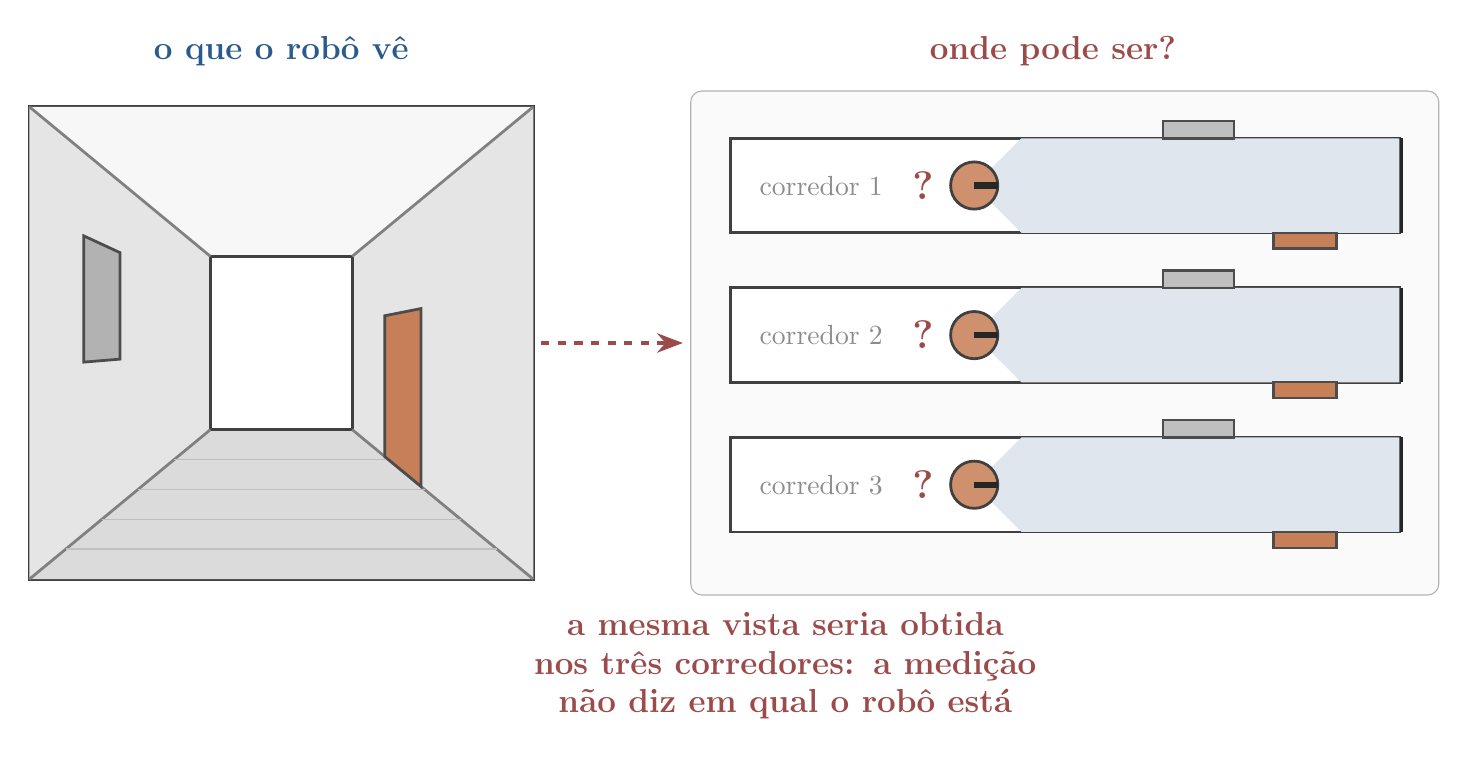
\begin{tikzpicture}[x=1cm,y=1cm,bal/.style={rectangle callout, rounded corners=7pt, draw=black!75, fill=white, line width=1pt, align=center, font=\normalsize, inner sep=5pt}]
  \newcommand{\robo}[3]{\begin{scope}[shift={(#1,#2)}, rotate=#3]\draw[black!75, fill=dorange!65, line width=1pt] (0,0) circle (0.32); \draw[black!85, line width=2.4pt, line cap=round] (0,0) -- (0.32,0);\end{scope}}

  % --- vista do robô (perspectiva) ---
  \node[font=\bfseries\large, dblue] at (3.2,6.7) {o que o robô \textbf{vê}};
  \draw[black!75, fill=black!6, line width=1.2pt] (0,0) rectangle (6.4,6.0);
  \fill[black!14] (0,0) -- (2.3,1.9) -- (4.1,1.9) -- (6.4,0) -- cycle;
  \fill[black!3] (0,6) -- (2.3,4.1) -- (4.1,4.1) -- (6.4,6) -- cycle;
  \fill[black!10] (0,0) -- (2.3,1.9) -- (2.3,4.1) -- (0,6) -- cycle;
  \fill[black!10] (6.4,0) -- (4.1,1.9) -- (4.1,4.1) -- (6.4,6) -- cycle;
  \draw[black!75, fill=white, line width=1pt] (2.3,1.9) rectangle (4.1,4.1);
  \draw[black!50, line width=1pt] (0,0) -- (2.3,1.9) (6.4,0) -- (4.1,1.9) (0,6.0) -- (2.3,4.1) (6.4,6.0) -- (4.1,4.1);
  % linhas do piso (profundidade)
  \foreach \t in {0.2,0.4,0.6,0.8} {\draw[black!25, line width=0.6pt] ({2.3*\t},{1.9*\t}) -- ({6.4-2.3*\t},{1.9*\t});}
  \draw[black!70, fill=black!30, line width=1pt] (0.690,2.757) -- (1.150,2.795) -- (1.150,4.148) -- (0.690,4.361) -- cycle;
  \fill[dorange!75] (4.974,1.178) -- (4.514,1.558) -- (4.514,3.346) -- (4.974,3.437) -- cycle; \draw[black!70, line width=1pt] (4.974,1.178) -- (4.514,1.558) -- (4.514,3.346) -- (4.974,3.437) -- cycle;

  % --- mapa visto de cima ---
  \node[font=\bfseries\large, dred] at (13.0,6.7) {onde \textbf{pode} ser?};
  \draw[black!30, fill=black!2, rounded corners=4pt] (8.4,-0.2) rectangle (17.9,6.2);
  \foreach \y/\n in {4.4/1,2.5/2,0.6/3} {
    \draw[black!75, fill=white, line width=1pt] (8.9,\y) rectangle (17.4,\y+1.2);
    \draw[black!85, line width=2.4pt] (17.4,\y) -- (17.4,\y+1.2);
    % campo de visão
    \fill[dblue!15] (12.0,\y+0.6) -- (12.6,\y+1.2) -- (17.4,\y+1.2) -- (17.4,\y) -- (12.6,\y) -- cycle;
    % quadro (parede esquerda = cima) e porta (parede direita = baixo)
    \draw[black!70, fill=black!25, line width=0.9pt] (14.4,\y+1.2) rectangle (15.3,\y+1.42);
    \fill[dorange!75] (15.8,\y-0.2) rectangle (16.6,\y); \draw[black!70, line width=0.8pt] (15.8,\y-0.2) rectangle (16.6,\y);
    \fill[dorange!65, draw=black!75, line width=1pt] (12.0,\y+0.6) circle (0.3); \draw[black!85, line width=2.2pt] (12.0,\y+0.6) -- (12.3,\y+0.6);
    \node[dred, font=\Large\bfseries] at (11.35,\y+0.6) {?};
    \node[dsub, font=\normalsize, anchor=west] at (9.15,\y+0.6) {corredor \n};
  }
  \draw[dred, dashed, line width=1.4pt, -{Stealth}] (6.5,3.0) -- (8.3,3.0);
  \node[font=\large\bfseries, dred, align=center, text width=9cm] at (9.6,-1.1) {a mesma vista seria obtida nos três corredores: a medição não diz em qual o robô está};
  \node[font=\small, dsub, align=left, anchor=west] at (8.9,6.65) {};
\end{tikzpicture}
\end{document}
